\documentclass[12pt,letterpaper]{article}
\usepackage{../pset_no_quiz_2024}

%Josh: add back in the commented out questions 
%note that I have left out the Team A question involving a causal explanation...seems too fraught philosohically perhaps! 


%Questions and Answers
\qa{q} % a="answers only"; q ="questions only"; b="both"
\usepackage{../qa}



\begin{document}

\psintro{Problem Set 3: Omega-Sequence Paradoxes}

%\com{ %following warning seems over-wrought here. most of the questions have straightforward answers
\question{
\fbox{\parbox{150mm}{\textbf{Note:} A murky problem can be addressed in more or less thoughtful ways. Good answers will reveal that you've understood the complexity of the underlying terrain and that you've given the issue serious thought.}}}

%Whereas problem Sets~1 and ~2 were largely a test of your math skills, Problem Set~3 will begin to test your philosophical abilities. In working through the problems, you may find that the rules of the game are not as clear as you'd like---and therefore that you can't just rely on your mathematical ability. 

\vspace{2mm}

%A murky problem can be addressed in more or less thoughtful ways. Good answers will reveal that you've understood the complexity of the underlying terrain and that you've given the issue serious thought. Addressing a murky question requires that you be \emph{more} rigorous, rather than less, because it's easier to make a mistake.}}}

%\subsection*{Part I} 


\begin{enumerate}

\item 
\question{  Lazy wants to run from \(A\) to \(B\), but he likes to take one-second breaks. He first stops halfway between \(A\) and \(B\) and takes a one-second break. He then stops halfway between that point and \(B\) and takes a one-second break, and so on. (More generally: for each  $k \geq 1$, Lazy takes a break at a distance of $(B-A)/2^k$ from $B$.) Assume that the traveling itself takes Lazy no time at all. Is there a positive integer \(n\) such that after \(n\) seconds Lazy has reached point \(B\)? If so, what is it? (10 points)}

\answer{No, there is no such positive integer \(n\). For suppose otherwise. Then there is some positive integer \(n\) such that Lazy will have reached \(B\) after \(n\) seconds. But that means she must have taken no more than \(n\) breaks. But after \(n\) breaks she will be at a distance from \(B\) of \((1/2^n)\) the distance between \(B\) and \(A\). So if Lazy takes no more than \(n\) breaks, then she cannot be any closer to \(B\) than \((1/2^n)\) the distance between \(B\) and \(A\).}

\item \question{

There are two prisoners in a room. They both close their eyes and each of
them is approached by a guard. Each guard flips a fair coin. If the coin lands Heads, she
gives her prisoner a red hat; if it lands Tails, she gives her prisoner a blue hat.
Once the prisoners have been assigned hats, they are both allowed to open their eyes.

As soon as they each see the color of the other's hat (but not the color of their own hat), the prisoners are taken into separate rooms and are unable to communicate with one another. At that point, they are each asked to name the color of their hat. %The prisoners must answer.
\begin{itemize}
\item if at least one of the prisoners answers correctly, they will both be set free;
\item otherwise, they will both remain in prison. Note that both MUST answer.
\end{itemize}
}

\begin{enumerate}
\item \question{Find a strategy that the prisoners can agree upon ahead of time which guarantees
that they are both set free.  Make sure your strategy is \emph{deterministic}: it must determine a definite outcome for each prisoner, given the prisoner's situation at the time of his decision. (8 points)}

\answer{Here's a strategy that guarantees success: Prisoner 1 picks the color of the other prisoner's hat; Prisoner 2 picks the color opposite to that of the other prisoner's hat.}

\item \question{Given that the prisoners have no access to information about the color of their own hats, and that the colors were chosen using independent coin tosses, what explains the possibility of a deterministic strategy that brings the prisoners' chance of freedom above 50\%? (12 points)}

\answer{The probability that a given prisoner answers correctly is no better than 50\%. (In fact, it is exactly 50\%.) But the strategy above guarantees that the prisoners' answers are \emph{coordinated}, so that one of them is right if and only if the other one is wrong. That's why the group's probability of success can go up to 1 even if the probability that each prisoner answers correctly is stuck at 50\%.}

\end{enumerate}

\item \question{Imagine an island on which everyone is either a knight or a knave. Knights only assert truths, knaves only assert falsehoods.  

For each of the scenarios below, determine whether one can settle the question of whether \(S_0\) is a knight or a knave. If the answer is ``yes'', state whether $S_0$ is a knight or a knave and explain how you know this; if the answer is ``no'', explain why.} 
%You may go over the word limit on part b

\begin{enumerate}

\item  \question{Ten islanders, \(S_0, S_1, \ldots, S_{9}\), are lined up. \(S_0\) is at the back; in front of her is \(S_1\); in front of him is \(S_2\); and so on. Each islander says: ``There is at least one person in front of me, and everyone in front of me is a knave.''  (10~points)}

\answer{  \(S_0\) is a knave. We know that \(S_9\) doesn't have anyone in front of her. So, \(S_9\) is lying---so \(S_9\) is a knave. So \(S_8\) speaks truly when he says, ``There is at least one person in front of me, and everyone in front of me is a knave." Since \(S_8\) is telling the truth, \(S_8\) must be a knight. But then we know that everyone else---\(S_7\), \(S_6\), \dots and \(S_0\)---are lying when they say ``There is at least one person in front of me, and everyone in front of me is a knave," since in front of all of them is one person who isn't a knave. Since \(S_0\) is lying, \(S_0\) is a knave.  }
 
\item   \question{An $\omega$-sequence of islanders,  \(S_0, S_1, S_2, \ldots\), are lined up.  \(S_0\) is still at the back of the line; in front of her is \(S_1\); in front of him is \(S_2\), and so on. Each islander says: 
``There is at least one person in front of me, and everyone in front of me is a knave.'' \textit{You may go over the word limit here}! (14~points)}

\answer{There is no coherent assignment of knight or knave status to \(S_0\). This problem is just Yablo's Paradox in disguise: it's just that we have island inhabitants instead of sentences.
      To see that no coherent assignment of knight or knave status is possible for \(S_0\), we will proceed by \emph{reductio}. We will first consider the assumption that \(S_0\) is a knight, and show that it leads to contradiction. We will then consider the assumption that \(S_0\) is a knave, and show that it too leads to contradiction.
      Suppose, first, that \(S_0\) is a knight. Then what she says is true. So it is true that there is at least one person in front of \(S_0\), and that everyone in front of her is a knave. That means, in particular, that \(S_1\) is a knave. So everything \(S_1\) says is false. So it is false that there is at least one person in front of \(S_1\) and that everyone in front of \(S_1\) is a knave. But since there are, in fact, people in front of \(S_1\), the only way for this to be false is for there to be some knight in front of \(S_0\), which contradicts the hypothesis that everything \(S_0\) says is true.
      Now suppose that \(S_0\) is a knave. Then what she says is false. So it is false that there is at least one person in front of \(S_0\) and that everyone in front of \(S_0\) is a knave. Since there are, in fact, people in front of \(S_0\), the only way for this to be false is for there to be some knight in front of \(S_0\). Say that that knight is \(S_k\). The same reasoning we used above to show that \(S_0\) cannot be a knight can be used to show that \(S_k\) cannot be a knight.
}
  
  

\item \question{As in the previous case, but this time each islander says: ``There is at least one person in front of me, and everyone in front of me is a knight.'' (14~points)}

\answer{It is consistent with the description of the problem that \(S_0\) be a knight, and consistent with the problem that \(S_0\) be a knave. 

It is consistent with the problem that everyone be a knight (and therefore that \(S_0\) be a knight). To see this, suppose that everyone is, indeed, a knight. Then for, any \(S_k\), it is true that there is at least one person in front of \(S_k\), and that everyone in front of \(S_k\) is a knight. So what \(S_k\) says is true. So \(S_k\) is indeed a knight. This means that our hypothesis that everyone is a knight is consistent with the description of the problem
 
 It is also consistent with the problem that everyone be a knave (and therefore that \(S_0\) be a knave). To see this, suppose that everyone is, indeed, a knave. Then for, any \(S_k\), it is false that everyone in front of \(S_k\) is a knight (and therefore false that there is at least one person in front of \(S_k\), \emph{and} that everyone in front of \(S_k\) is a knight). So what \(S_k\) says is false. So \(S_k\) is indeed a knave. This means that our hypothesis that everyone is a knave is consistent with the description of the problem}


\end{enumerate}




\com{ %2023 decided to leave this out after all, since could cause a headache for grading!
\item \question{
There are countably many assassins ready to kill Oscar, should he attempt to enter the room:}


\begin{itemize}
\item  Assassin 1 will kill Oscar if and only if Oscar is still alive when any part of his body crosses the threshold of the room by more than 1 mm. 

\item Assassin 2 will kill Oscar if and only if Oscar is still alive when any part of his body crosses the threshold of the room by more than 1/2 mm. 

\hspace{50mm} {\vdots}

\item Assassin $n$ will kill Oscar if and only if Oscar is still alive when any part of his body crosses the threshold of the room by more than 1/$n$ mm. 

\hspace{50mm} {\vdots}

\end{itemize}
All assassins kill instantly if they kill at all. On the assumption that Oscar can only die if he's killed by someone, is it possible for him to cross the threshold? Possible for him to cross the threshold and remain alive? If not, what stops him?  (10 points; don't forget about the word limit.)
%}

\answer{What I'm looking for here is some awareness of the fact that the situation is paradoxical. An especially good answer would suggest a sensible way out of the paradox. (It might say, for example, that in any world with the relevant setup Oscar fails to enter the room, and therefore that it is impossible for him to enter the room given the setup.)}
}


\item \question{The following questions are intended to test your understanding of continuity assumptions. At least one of them might get into ``murky'' territory. If you think there is a \textit{determinate way} the wheel will look or direction a line will point, explain why. \\ If instead you think that the way the wheel will look or where a line will point is \textit{undetermined} by the scenario described, explain why.}

%They may or may not have determinate answers. (If you think a question has a determinate answer, make sure you explain why. If you think it doesn't, make sure you explain why not.)}%\footnote{Rayo was told that the underlying puzzle was created by Frank Arntzenius's daughter, when she was very little.}

\begin{enumerate}
	
	\item \question{
	You have a wheel with a radius of 1 unit. You draw a red line going from the center of the wheel to the twelve o'clock position:
	
\begin{center}
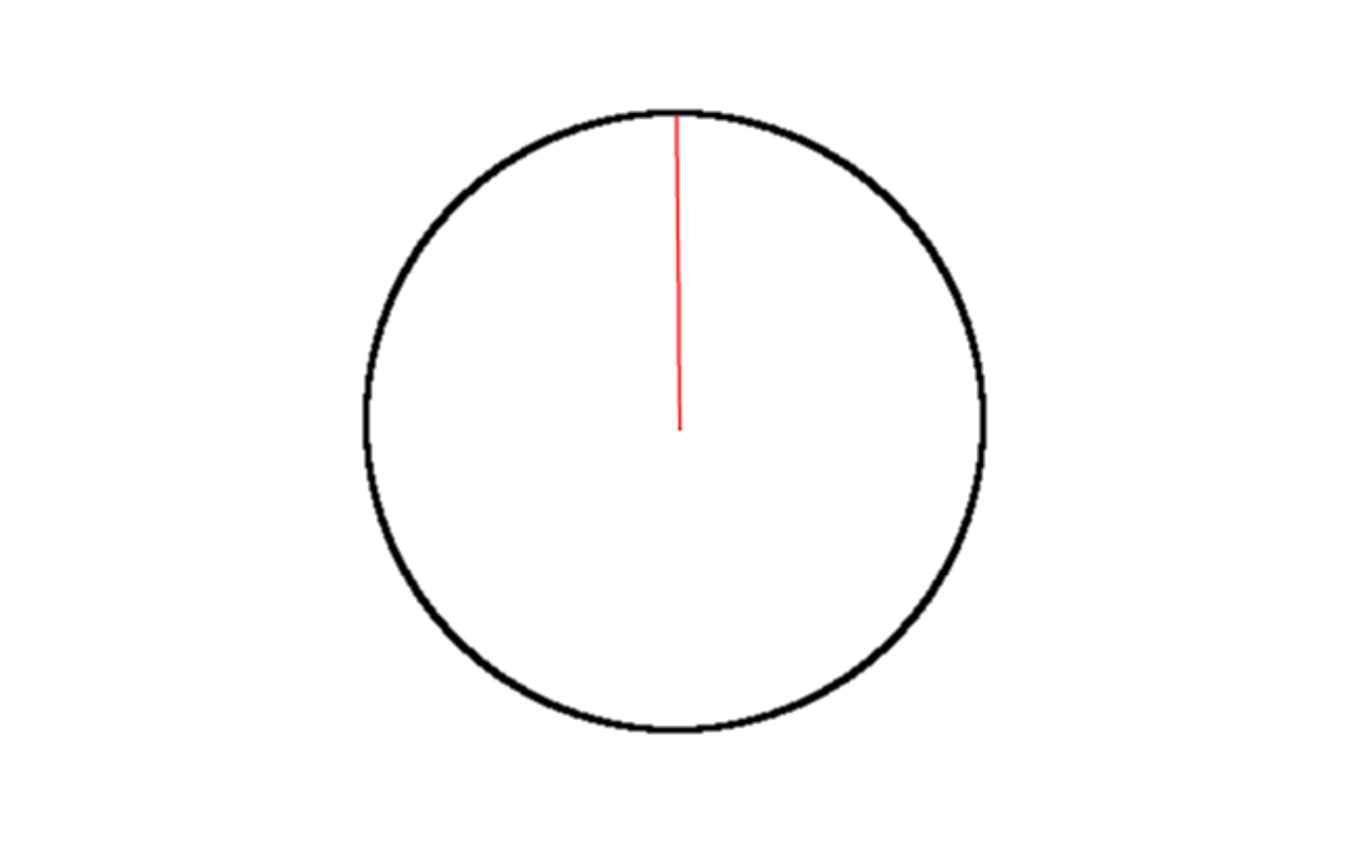
\includegraphics[scale=.2]{base}
\end{center}
	
	 You then rotate the wheel, in steps. At each step, you rotate the wheel one radian clockwise, so that the outermost point of the red line travels 1 unit around the perimeter of the wheel. Here is the first rotation:
	
	\begin{center}
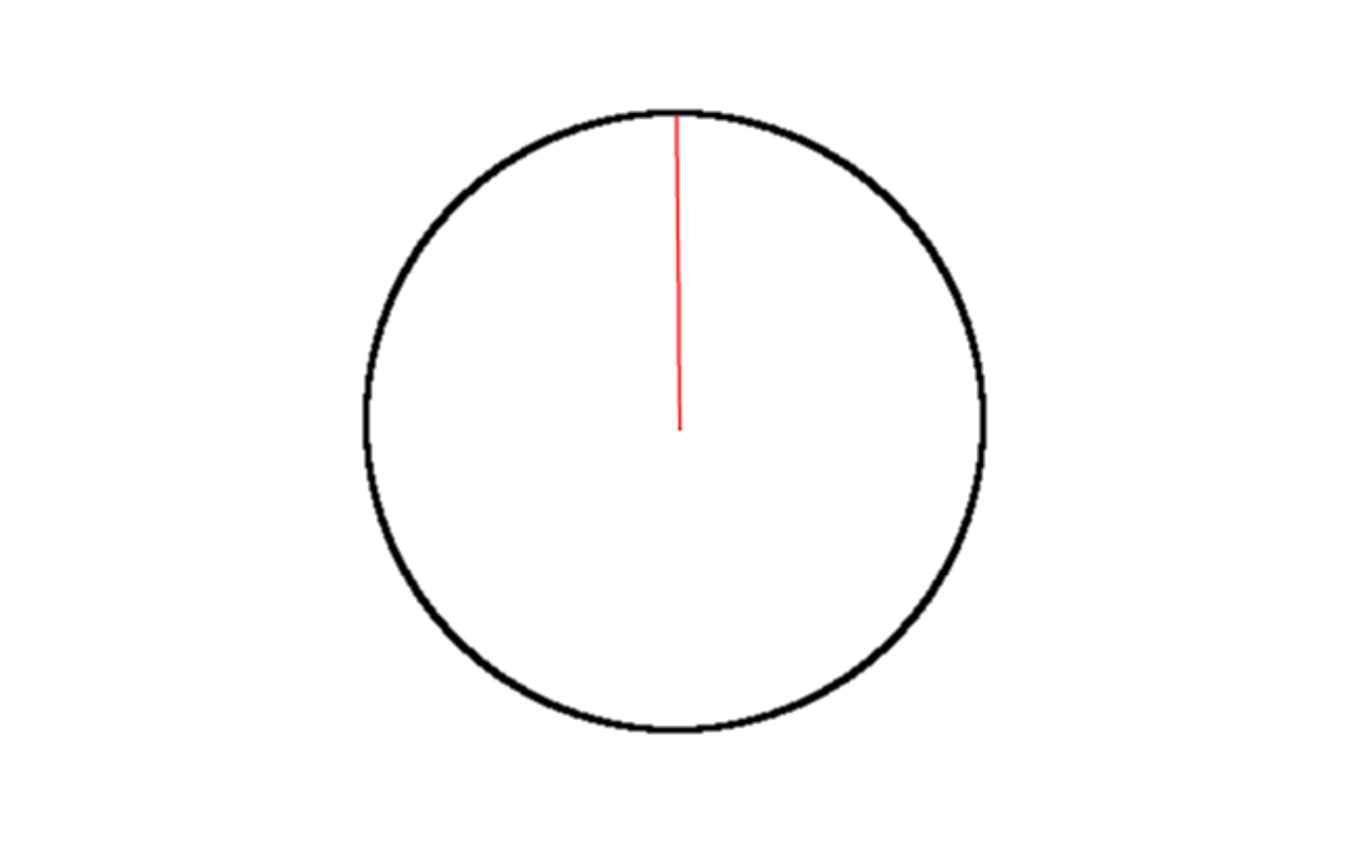
\includegraphics[scale=.2]{base}  \raisebox{13mm}{$\longrightarrow$} 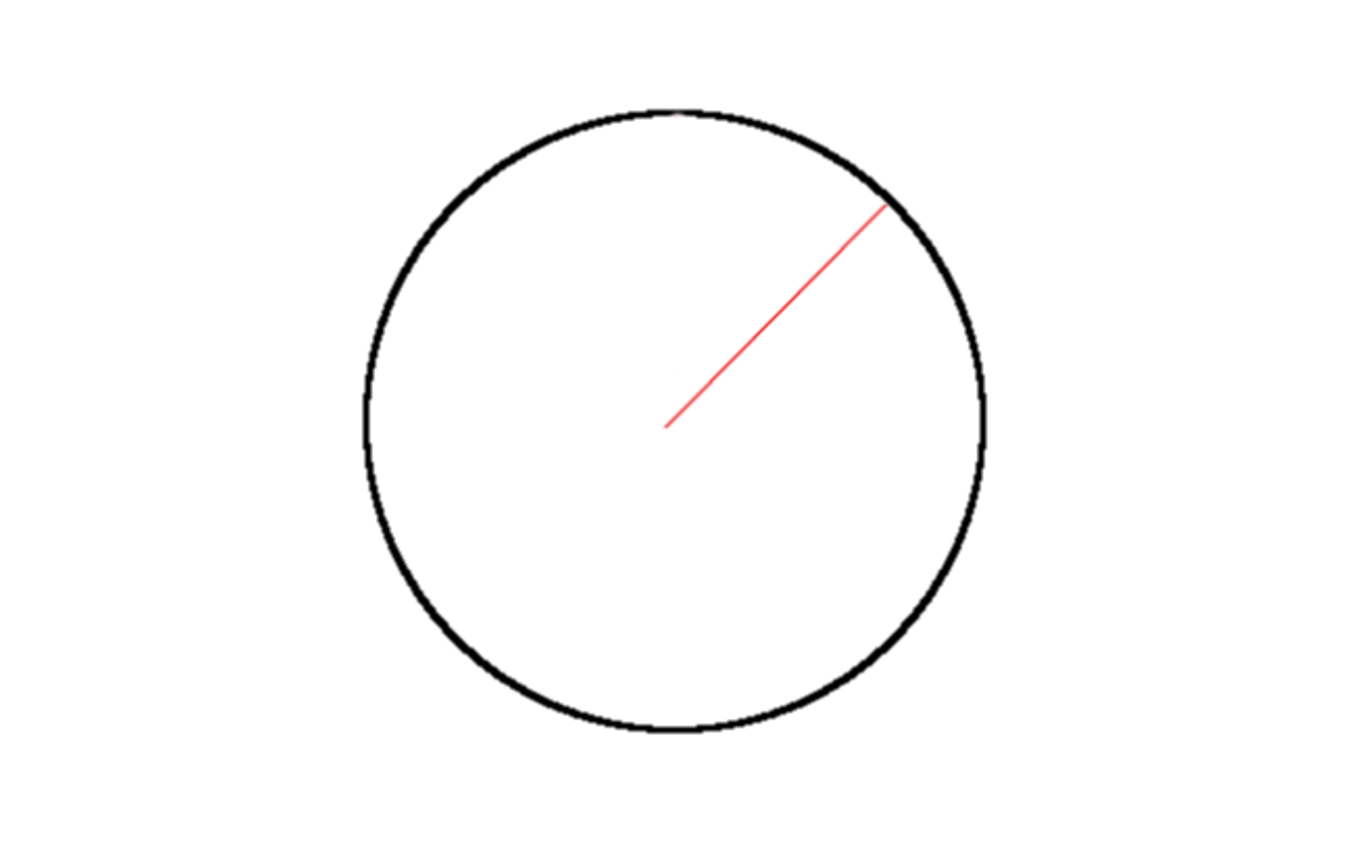
\includegraphics[scale=.2]{1rad}
\end{center}
Because the tip of the red line travels 1 unit around the perimeter after each rotation, and because the perimeter of the wheel is $2\pi$ units (which is an irrational number of units), there is no positive integer $n$ such that, after $n$ steps, the red line returns to a position it had occupied before.

Suppose you perform this operation infinitely many times, once for each positive integer. At noon the red line is at the twelve o'clock position. At 12:30 you rotate the wheel one radian clockwise. At 12:45 you rotate the wheel another radian clockwise. And so forth: for each $n \geq 1$, you perform the $n$th rotation $\frac{1}{2^n}$ hours before 1pm.

\textbf{Question}: in which direction will the red line be pointing at 1pm? Don't forget to justify your answer. (10 points)}

\answer{The answer is not determined by the description of the problem.}


\item \question{
Consider a variant of the case in part (a). As before, you start by drawing a red line from the center of the wheel to the twelve o'clock position. But this time you draw new lines, in steps. At each step, you draw a red line at a one radian angle from the last line you drew. At noon you draw the initial red line, pointing to the twelve o'clock position. At 12:30 you draw an additional line, a radian away in the clockwise direction. At 12:45 you draw an additional line, a radian away in the clockwise direction. And so forth: for each $n \geq 1$, you draw a line $\frac{1}{2^n}$ hours before 1pm. Here are the first two steps of the process:


	\begin{center}
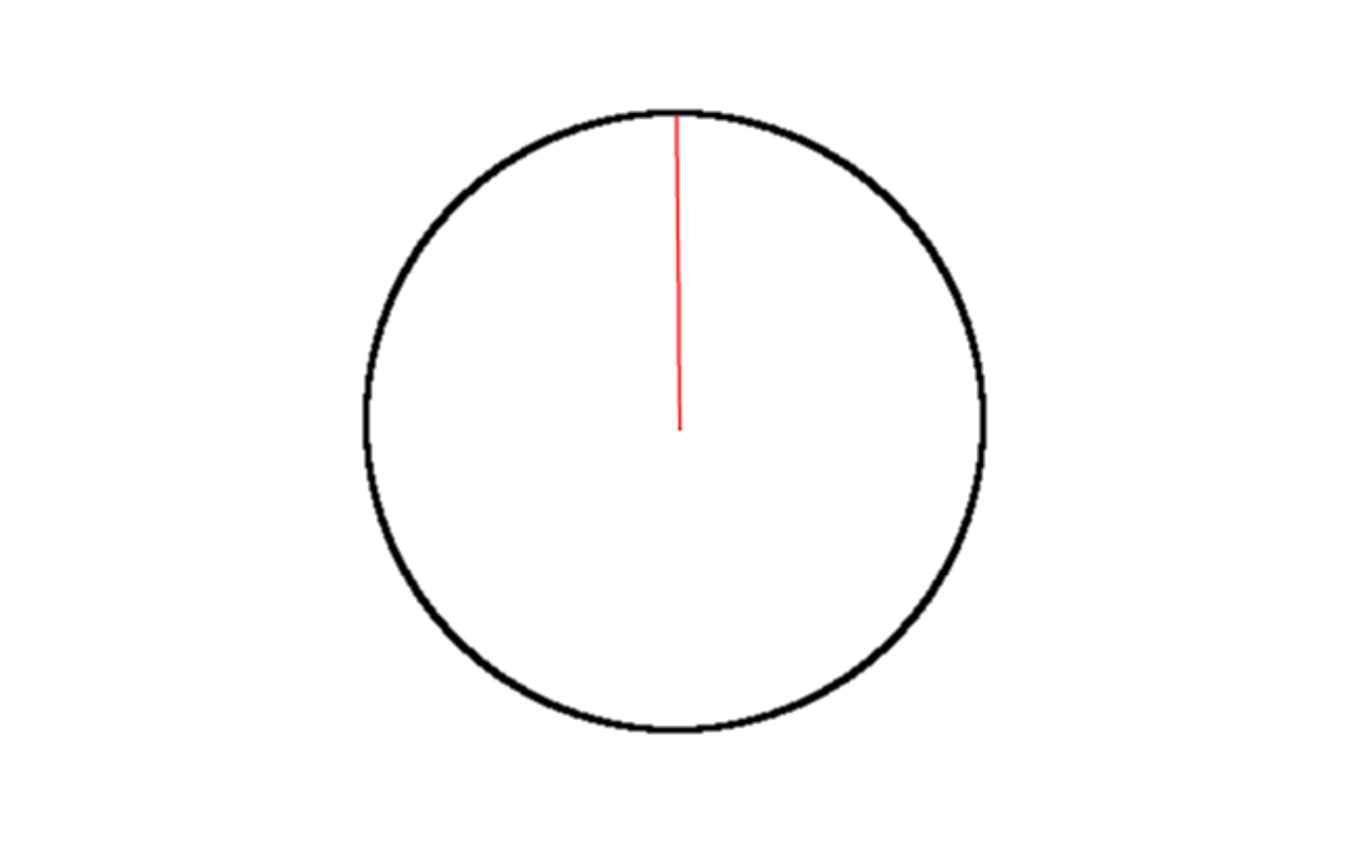
\includegraphics[scale=.2]{base}  \raisebox{13mm}{$\longrightarrow$} 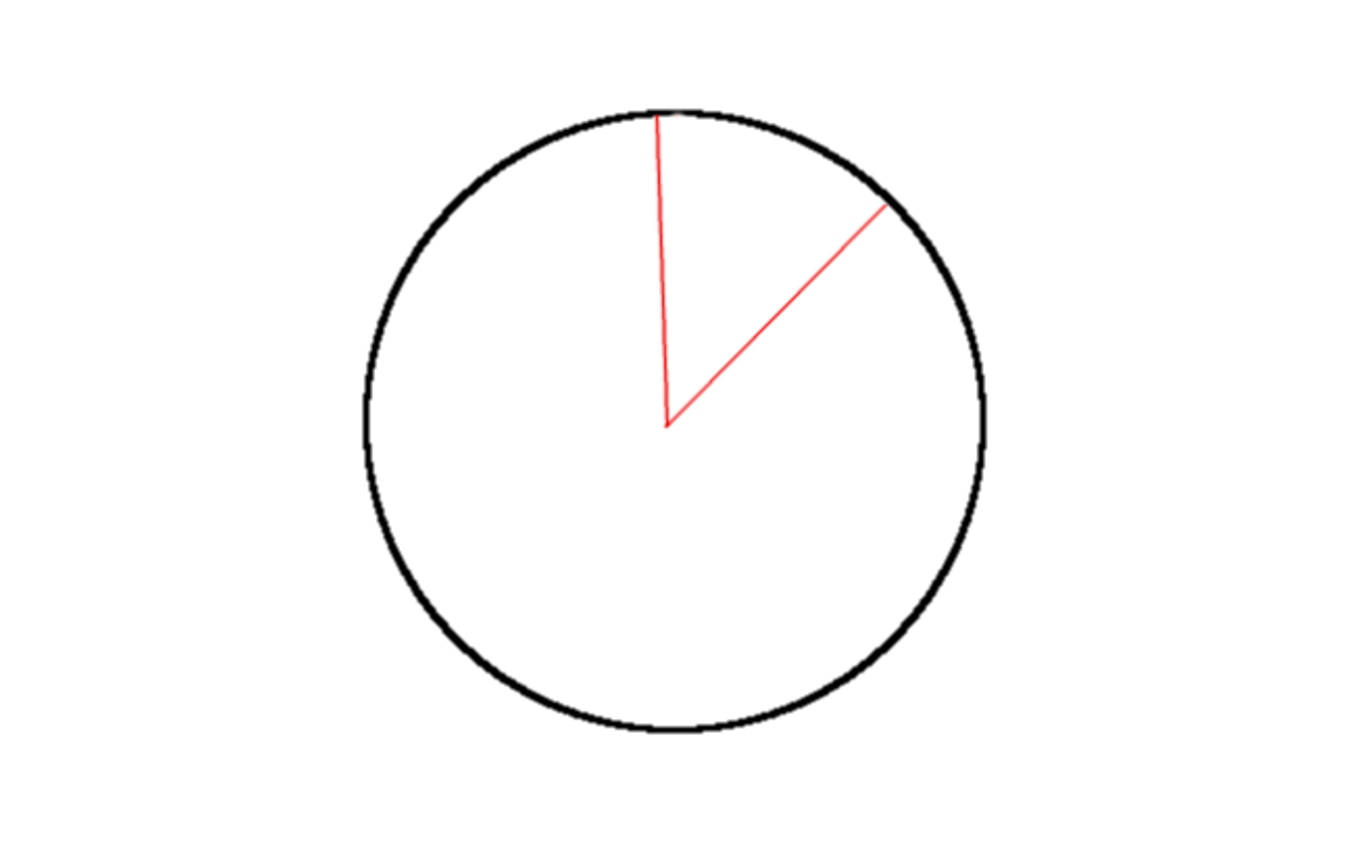
\includegraphics[scale=.2]{2rad}
\end{center}



At 1pm, you're done drawing lines on the wheel. Note that there's a well-defined fact of the matter about what the wheel is like. Namely: a radial line $r$ will be colored red if and only if, for some number $n$, $r$ is exactly $n$ radians away from twelve o'clock, going clockwise.


The next step is to rotate the wheel. Consider the result of rotating the wheel one radian in the clockwise direction. It'll look exactly the way the unrotated wheel would have looked  if you had skipped drawing the 12pm line. And if you rotate the wheel one radian further, for a total rotation of two radians,  it'll look exactly the way the unrotated wheel would have looked  if you had skipped drawing the 12pm and 12:30pm lines. And so forth: after a total of $n$ rotations, the wheel will look exactly the way the original unrotated wheel would have looked  if you had skipped drawing all lines up to and including the 1pm$-\frac{1}{2^{n-1}}$ hours line.

Suppose that you rotate the wheel infinitely many times, once for each positive integer. At 1pm you rotate the wheel one radian in the clockwise direction. At 1:30 you rotate the wheel another radian in the clockwise direction. Again at 1:45. And so forth. For each $n \geq 0$, you perform the $n$th rotation $\frac{1}{2^n}$ hours before 2:00pm. 

\textbf{Question}: What does the wheel look like at 2pm? Assume that the only way for a line to disappear is for someone to erase it. (12 points)
}


\answer{One excellent answer is to say that the wheel looks exactly the way it did before you started rotating. (Some students might add that the description of the problem doesn't settle the wheel's orientation, but failure to do so shouldn't be penalized.)}


\item \question{Suppose you start by drawing lines on the wheel as in part (b). But this time you perform no rotations. Instead, you \emph{erase} red lines using the following procedure. At 1:00pm you erase the red line pointing to the twelve o'clock position. At 1:30 you erase the line pointing one radian in the clockwise direction from the last line erased. And so forth: for each $n \geq 1$, you erase the line one radian away in the clockwise direction from the last line erased.

\textbf{Question}: Is there a difference between the way our wheel looks at 2pm and the way the wheel in the previous exercise looked at 2pm? Assume that the only way for an erased line to reappear is for someone to redraw it. (10~points)}

\answer{Yes, there is a difference. In the case in which you erase lines, the wheel will be completely unmarked at 2pm.}


\end{enumerate}
  

\end{enumerate}

%\end{enumerate}

\end{document}
